% Study 2, the secondary tables of the appendix, from the inference and post-hoc files of the two runs and
% the post-hoc dynamic-occurrence directory. Input from paper.tex; every number traces to sources.md and is
% asserted by check_numbers.py.
\providecommand{\lm}{\texttt{local\_mean\_28}}
\providecommand{\aets}{\texttt{autoets\_weekly}}
\providecommand{\qs}{QScore9}
\providecommand{\hc}{\texttt{hurdle\_count\_28}}

\section{Study 2: the two families, the secondary tables and the post-hoc readings}
\label{app:s2tables}

Tables~\ref{tab:s2ext} and~\ref{tab:s2syn} give the two registered families of Study 2 with every column,
the eighteen external comparisons on the npm panel and the six synthetic comparisons at horizon 30;
Figure~\ref{fig:s2npm} shows the 209 paired differences behind each external row, and
Table~\ref{tab:s2parts} splits each hurdle-minus-control difference into the three exact accounting parts.
Twelve of the eighteen external tests and five of the six synthetic tests reject at $q = 0.05$ after one
adjustment per family; of the twelve, ten reject for the model variant and two against it, and all five
synthetic rejections are against the hurdle variant. None of the other tables in this appendix carries a
multiplicity adjustment except the two post-hoc dynamic-occurrence families, which carry their own, and
none replaces the two families. Differences are model variant minus reference, so negative favors the
variant. A median of order $10^{-9}$ is a near-zero score difference repeated across series, not a tie; under
the declared rule only an exact zero is a tie.

\begin{table}[htbp]
\centering\footnotesize\setlength{\tabcolsep}{3pt}
\caption{The eighteen declared external comparisons on the npm panel. Differences are model variant minus
reference \qs{}, averaged over three origins within series and then over 209 series; negative favors the
variant. The contrast names the pair: the model's hurdle against its completed control, the hurdle against
\hc{}, or the raw deciles against \lm{} (the full tuples are in Appendix Table~\ref{tab:s2family}). The
interval is the pointwise 95 percent percentile interval from 20,000 series-cluster bootstrap replicates.
``Lower / tied / higher'' counts the series (of 209) where the variant's score is below, equal to or above
the reference's. $p$ is the Benjamini-Hochberg adjusted two-sided Wilcoxon signed-rank $p$-value over the
18 tests. Every mean in this table is carried by the series \texttt{aggregate-error}
(Appendix~\ref{app:s2panel}); the medians, counts and tests are rank-based and describe the typical series.}
\label{tab:s2ext}
\begin{tabular}{lllrrcrcl}
\toprule
ID & Model & Contrast & $h$ & Mean & 95\% interval & Median & Lower / tied / higher & Adjusted $p$ \\
\midrule
E01 & Chronos-2 & hurdle vs completed & 7 & 152 & [0.1846, 455.2] & -0.01376 & 121 / 2 / 86 & 0.203 \\
E02 & Chronos-2 & hurdle vs count hurdle & 7 & -5,090 & [-15,175, -31.08] & -0.01587 & 129 / 12 / 68 & $3.72 \times 10^{-11}$ \\
E03 & Chronos-2 & raw vs local mean & 7 & -2,884 & [-8,601, -17.33] & 0.007856 & 92 / 0 / 117 & 0.596 \\
E04 & Chronos-2 & hurdle vs completed & 30 & 90.24 & [0.2273, 269.7] & -0.0002469 & 105 / 2 / 102 & 0.449 \\
E05 & Chronos-2 & hurdle vs count hurdle & 30 & -6,563 & [-19,596, -30.03] & -0.06173 & 150 / 9 / 50 & $7.06 \times 10^{-21}$ \\
E06 & Chronos-2 & raw vs local mean & 30 & -4,734 & [-14,149, -15.84] & -0.002372 & 112 / 0 / 97 & 0.0119 \\
E07 & TimesFM 3 & hurdle vs completed & 7 & 176.9 & [0.2669, 529.4] & 0.001058 & 94 / 8 / 107 & 0.236 \\
E08 & TimesFM 3 & hurdle vs count hurdle & 7 & -5,416 & [-16,153, -31.67] & -0.007407 & 116 / 18 / 75 & $3.61 \times 10^{-8}$ \\
E09 & TimesFM 3 & raw vs local mean & 7 & -3,235 & [-9,650, -18.24] & -0.002297 & 112 / 1 / 96 & 0.0438 \\
E10 & TimesFM 3 & hurdle vs completed & 30 & 128.5 & [0.5058, 383.8] & 0.00321 & 81 / 8 / 120 & 0.00215 \\
E11 & TimesFM 3 & hurdle vs count hurdle & 30 & -6,792 & [-20,280, -31.3] & -0.0716 & 161 / 17 / 31 & $3.19 \times 10^{-25}$ \\
E12 & TimesFM 3 & raw vs local mean & 30 & -5,001 & [-14,947, -16.86] & -0.005016 & 125 / 1 / 83 & $3.82 \times 10^{-5}$ \\
E13 & TimesFM 2.5 & hurdle vs completed & 7 & 253.9 & [0.5046, 759.9] & -0.002116 & 109 / 3 / 97 & 0.628 \\
E14 & TimesFM 2.5 & hurdle vs count hurdle & 7 & -5,847 & [-17,446, -30.83] & -0.006349 & 115 / 7 / 87 & $2.66 \times 10^{-5}$ \\
E15 & TimesFM 2.5 & raw vs local mean & 7 & -3,743 & [-11,179, -17.41] & 0.01696 & 84 / 1 / 124 & 0.746 \\
E16 & TimesFM 2.5 & hurdle vs completed & 30 & 110.3 & [0.6883, 328.7] & 0.0009877 & 101 / 1 / 107 & 0.0276 \\
E17 & TimesFM 2.5 & hurdle vs count hurdle & 30 & -6,918 & [-20,665, -29.9] & -0.06938 & 160 / 9 / 40 & $1.77 \times 10^{-23}$ \\
E18 & TimesFM 2.5 & raw vs local mean & 30 & -5,109 & [-15,279, -15.49] & -0.003695 & 113 / 1 / 95 & 0.00204 \\
\bottomrule
\end{tabular}
\end{table}

\begin{table}[htbp]
\centering\footnotesize\setlength{\tabcolsep}{3pt}
\caption{The six declared synthetic comparisons at horizon 30. Differences are model variant minus reference
\qs{}, averaged over three origins within each replicate and cell, then over the 18 cells with equal weight,
so that each of the 30 replicate blocks carries one paired difference; negative favors the variant. The
interval is the pointwise 95 percent percentile interval from 20,000 replicate-block bootstrap replicates.
``Lower / tied / higher'' counts the blocks (of 30) where the variant's score is below, equal to or above
the reference's. $p$ is the Benjamini-Hochberg adjusted two-sided Wilcoxon signed-rank $p$-value over the
6 tests.}
\label{tab:s2syn}
\begin{tabular}{lllrrcrcl}
\toprule
ID & Model & Contrast & $h$ & Mean & 95\% interval & Median & Lower / tied / higher & Adjusted $p$ \\
\midrule
S01 & Chronos-2 & hurdle vs completed & 30 & 0.08599 & [0.03836, 0.1401] & 0.05554 & 6 / 0 / 24 & 0.00415 \\
S02 & Chronos-2 & hurdle vs count hurdle & 30 & 0.05211 & [0.01686, 0.09227] & 0.04737 & 9 / 0 / 21 & 0.0111 \\
S03 & TimesFM 3 & hurdle vs completed & 30 & 0.08662 & [0.03837, 0.1429] & 0.06144 & 6 / 0 / 24 & 0.00676 \\
S04 & TimesFM 3 & hurdle vs count hurdle & 30 & 0.0215 & [-0.006569, 0.04947] & 0.03119 & 11 / 0 / 19 & 0.12 \\
S05 & TimesFM 2.5 & hurdle vs completed & 30 & 0.08769 & [0.04316, 0.1382] & 0.06743 & 5 / 0 / 25 & 0.00415 \\
S06 & TimesFM 2.5 & hurdle vs count hurdle & 30 & 0.06109 & [0.02299, 0.09881] & 0.06027 & 9 / 0 / 21 & 0.00798 \\
\bottomrule
\end{tabular}
\end{table}

\begin{figure}[htbp]
\centering
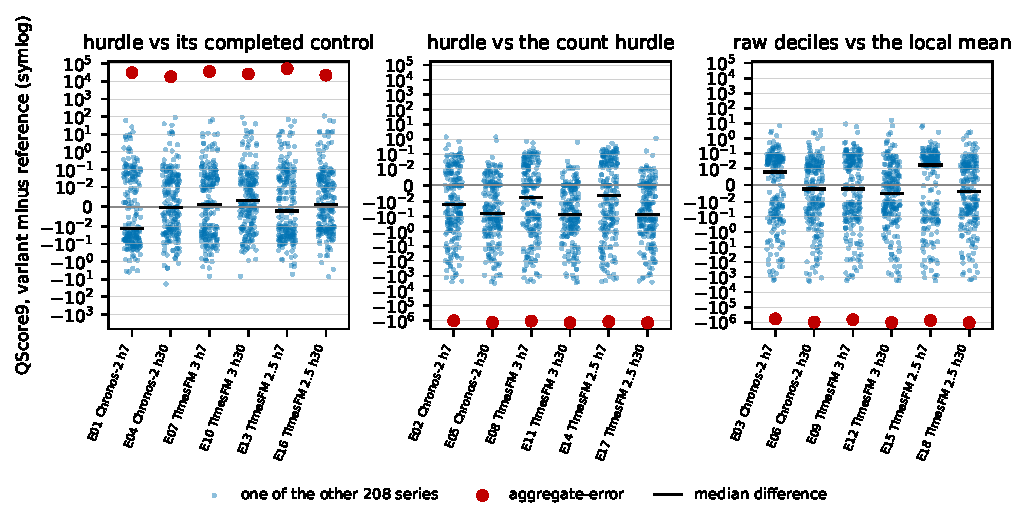
\includegraphics[width=\textwidth]{fig-s2-npm-paired-differences}
\caption{The eighteen external comparisons, series by series. Each point is one of the 209 series' paired
difference (variant minus reference \qs{}, three origins averaged) on a symmetric log scale, grouped by
contrast; the filled red marker is \texttt{aggregate-error}, and the short bar is the median. The mean of
each row, in Table~\ref{tab:s2ext}, is the red marker's value divided by 209 plus a remainder of a different
order.}
\label{fig:s2npm}
\end{figure}

\begin{table}[htbp]
\centering\small
\caption{The hurdle-minus-control difference (E01, E04, E07, E10, E13, E16 on npm; S01, S03, S05 on the
grid) and its three exact accounting parts, each divided by the full horizon: the loss on zero target days,
the loss on positive days from quantiles above the target (overprediction) and from quantiles below it
(underprediction). Equal-series and equal-block means; the parts sum to the total. Negative favors the
hurdle. The npm parts are unscaled and \texttt{aggregate-error} dominates them.}
\label{tab:s2parts}
\begin{tabular}{llrrrrr}
\toprule
Study & Model & $h$ & Total & Zero days & Positive, overprediction & Positive, underprediction \\
\midrule
npm & Chronos-2 & 7 & 152 & -0.3176 & -161.7 & 314 \\
npm & TimesFM 3 & 7 & 176.9 & -0.3701 & -149.5 & 326.8 \\
npm & TimesFM 2.5 & 7 & 253.9 & -0.3425 & -91.81 & 346 \\
npm & Chronos-2 & 30 & 90.24 & -63.79 & -146.1 & 300.1 \\
npm & TimesFM 3 & 30 & 128.5 & -66.08 & -112.9 & 307.5 \\
npm & TimesFM 2.5 & 30 & 110.3 & -67.09 & -131.9 & 309.4 \\
synthetic & Chronos-2 & 30 & 0.08599 & -0.1752 & -0.03194 & 0.2931 \\
synthetic & TimesFM 3 & 30 & 0.08662 & -0.172 & -0.0282 & 0.2868 \\
synthetic & TimesFM 2.5 & 30 & 0.08769 & -0.2293 & -0.03873 & 0.3557 \\
\bottomrule
\end{tabular}
\end{table}

\paragraph{By stratum.} The strata are declared secondary descriptors and carry no interval and no test;
the very sparse stratum holds $n = 9$ series, not 100. Against its completed control the hurdle variant
scores lower on 32 to 43 of the 100 dense series across the six cells, on 45 to 81 of the 100 sparse
series, and on 2 to 4 of the 9 very sparse series, where the median difference is exactly 0 in five of the
six cells. Against \hc{} it scores lower on 80 to 94 of the 100 dense series, on 29 to 63 of the 100 sparse
series and on 4 of the 9 very sparse series in every cell, with a median of exactly 0 there in all six. The
raw deciles score lower than \lm{} on 61 to 70 dense, 19 to 51 sparse and 4 or 5 very sparse series. With
nine series the very sparse stratum supports no reading beyond those counts (Table~\ref{tab:s2strata}).
Table~\ref{tab:s2regime} adds, post hoc and with no registered status, the lower-tied-higher counts, the
median and a raw two-sided signed-rank $p$ for the hurdle against its control within each stratum, computed
from the saved per-series scores; Table~\ref{tab:s2empirical} does the same for the hurdle against the
registered secondary \texttt{hurdle\_empirical\_28} by stratum and for the completed control against it
over all 209 series. A signed-rank test restricted to each stratum, computed post hoc from the saved per-series scores and
adding no registered test (Table~\ref{tab:s2regime}), has raw $p$ below 0.002 for all three
sparse-stratum contrasts at horizon 7 and from 0.47 to 0.892 at horizon 30. On the grid, by zero
probability, the hurdle beats its control in 4 to 6 of 30 replicate blocks at $z = 0.2$, in 12 to 15 at
$z = 0.8$ and in 21 to 26 at $z = 0.95$ (Table~\ref{tab:s2cells}). The dense result has a mechanical
cause: a series with no zero in its last 28 context days gets $p = 28.5 / 29$, so the hurdle forces about
1.7 percent of mass onto zero on every day, where the model's own completed law, which puts less there,
must win.

\begin{table}[htbp]
\centering\scriptsize\setlength{\tabcolsep}{2.4pt}
\caption{Post-hoc. The hurdle variant against its completed control within each stratum: ``L / T / H'', the
series where the hurdle is lower, tied or higher; the median difference; and the raw two-sided signed-rank
$p$ with zero differences omitted, computed from the saved per-series scores; no adjustment, no registered
status. The very sparse stratum holds $n = 9$.}
\label{tab:s2regime}
\begin{tabular}{llcrlcrlcrl}
\toprule
 & & \multicolumn{3}{c}{dense, $n = 100$} & \multicolumn{3}{c}{sparse, $n = 100$} & \multicolumn{3}{c}{very sparse, $n = 9$} \\
\cmidrule(lr){3-5} \cmidrule(lr){6-8} \cmidrule(lr){9-11}
Model & $h$ & L / T / H & Median & Raw $p$ & L / T / H & Median & Raw $p$ & L / T / H & Median & Raw $p$ \\
\midrule
Chronos-2 & 7 & 36 / 0 / 64 & 0.0455 & 0.0055 & 81 / 1 / 18 & -0.03333 & $2.47 \times 10^{-11}$ & 4 / 1 / 4 & 0 & 0.297 \\
TimesFM 3 & 7 & 32 / 0 / 68 & 0.03386 & 0.000363 & 60 / 3 / 37 & -0.009524 & 0.00158 & 2 / 5 / 2 & 0 & 0.625 \\
TimesFM 2.5 & 7 & 40 / 0 / 60 & 0.03386 & 0.00241 & 66 / 2 / 32 & -0.01058 & $9.01 \times 10^{-5}$ & 3 / 1 / 5 & 0.007407 & 0.82 \\
Chronos-2 & 30 & 43 / 0 / 57 & 0.01543 & 0.144 & 58 / 1 / 41 & -0.003086 & 0.47 & 4 / 1 / 4 & 0 & 0.312 \\
TimesFM 3 & 30 & 34 / 0 / 66 & 0.02173 & 0.000636 & 45 / 4 / 51 & 0.0004938 & 0.65 & 2 / 4 / 3 & 0 & 0.438 \\
TimesFM 2.5 & 30 & 43 / 0 / 57 & 0.02333 & 0.00106 & 54 / 0 / 46 & -0.0008642 & 0.892 & 4 / 1 / 4 & 0 & 0.312 \\
\bottomrule
\end{tabular}
\end{table}

\begin{table}[htbp]
\centering\footnotesize\setlength{\tabcolsep}{3.5pt}
\caption{Post-hoc. The foundation-model hurdle against the registered secondary
\texttt{hurdle\_empirical\_28}, which shares its occurrence rule and uses the empirical positive law, by
stratum (series where the hurdle is lower, tied or higher); and the completed control against the same
empirical hurdle over all 209 series, with the median difference and the raw two-sided signed-rank $p$.
Computed from the saved per-series scores; no adjustment, no registered status.}
\label{tab:s2empirical}
\begin{tabular}{llcccccl}
\toprule
 & & \multicolumn{3}{c}{hurdle vs empirical hurdle, lower / tied / higher} & \multicolumn{3}{c}{completed vs empirical hurdle, $n = 209$} \\
\cmidrule(lr){3-5} \cmidrule(lr){6-8}
Model & $h$ & dense, $n = 100$ & sparse, $n = 100$ & very sparse, $n = 9$ & Lower / tied / higher & Median & Raw $p$ \\
\midrule
Chronos-2 & 7 & 65 / 0 / 35 & 50 / 8 / 42 & 4 / 4 / 1 & 88 / 2 / 119 & 0.01058 & 0.598 \\
TimesFM 3 & 7 & 64 / 1 / 35 & 45 / 10 / 45 & 4 / 4 / 1 & 117 / 5 / 87 & -0.006349 & 0.00804 \\
TimesFM 2.5 & 7 & 63 / 0 / 37 & 33 / 3 / 64 & 4 / 4 / 1 & 90 / 1 / 118 & 0.009524 & 0.478 \\
Chronos-2 & 30 & 66 / 0 / 34 & 45 / 4 / 51 & 6 / 3 / 0 & 120 / 3 / 86 & -0.00716 & $4.94 \times 10^{-5}$ \\
TimesFM 3 & 30 & 68 / 0 / 32 & 55 / 13 / 32 & 5 / 4 / 0 & 140 / 8 / 61 & -0.01037 & $1.22 \times 10^{-8}$ \\
TimesFM 2.5 & 30 & 72 / 1 / 27 & 57 / 4 / 39 & 5 / 4 / 0 & 130 / 1 / 78 & -0.01012 & $5.1 \times 10^{-7}$ \\
\bottomrule
\end{tabular}
\end{table}

\begin{table}[htbp]
\centering\footnotesize\setlength{\tabcolsep}{3.5pt}
\caption{The context-scaled \qs{}, the registered scale-free secondary: each window's \qs{} divided by
$\max(1, \bar{y}_{\text{context}})$ before the registered averaging. Mean difference with its pointwise 95
percent bootstrap interval, median difference, and ``L / T / H'', the series (of 209) or blocks (of 30)
where the variant is lower, tied or higher. The synthetic rows are at horizon 30; the suffix \texttt{-h7}
marks the horizon-7 secondary rows.}
\label{tab:s2scaled}
\begin{tabular}{lllrrcrc}
\toprule
ID & Variant & Reference & $h$ & Mean & 95\% interval & Median & L / T / H \\
\midrule
E01 & chronos2\_hurdle & chronos2\_completed & 7 & -0.02204 & [-0.03098, -0.01407] & -0.005825 & 122 / 2 / 85 \\
E04 & chronos2\_hurdle & chronos2\_completed & 30 & -0.002395 & [-0.006836, 0.00146] & 0.0002262 & 101 / 2 / 106 \\
E02 & chronos2\_hurdle & hurdle\_count\_28 & 7 & -0.1311 & [-0.1809, -0.08701] & -0.01058 & 129 / 12 / 68 \\
E05 & chronos2\_hurdle & hurdle\_count\_28 & 30 & -0.1456 & [-0.1909, -0.1055] & -0.02617 & 150 / 9 / 50 \\
E03 & chronos2\_raw & local\_mean\_28 & 7 & -0.01511 & [-0.03735, 0.004919] & 0.003944 & 92 / 0 / 117 \\
E06 & chronos2\_raw & local\_mean\_28 & 30 & -0.02913 & [-0.04976, -0.01305] & -0.00184 & 112 / 0 / 97 \\
E07 & timesfm3\_hurdle & timesfm3\_completed & 7 & -0.006708 & [-0.01467, -0.0001148] & 0.0008949 & 95 / 8 / 106 \\
E10 & timesfm3\_hurdle & timesfm3\_completed & 30 & 0.001291 & [-0.001255, 0.003757] & 0.001769 & 80 / 8 / 121 \\
E08 & timesfm3\_hurdle & hurdle\_count\_28 & 7 & -0.1278 & [-0.1761, -0.08451] & -0.004233 & 116 / 18 / 75 \\
E11 & timesfm3\_hurdle & hurdle\_count\_28 & 30 & -0.1466 & [-0.19, -0.1075] & -0.03038 & 161 / 17 / 31 \\
E09 & timesfm3\_raw & local\_mean\_28 & 7 & -0.02463 & [-0.04487, -0.007124] & -0.001849 & 112 / 1 / 96 \\
E12 & timesfm3\_raw & local\_mean\_28 & 30 & -0.03336 & [-0.05248, -0.01843] & -0.003988 & 124 / 1 / 84 \\
E13 & timesfm2p5\_hurdle & timesfm2p5\_completed & 7 & -0.006123 & [-0.01111, -0.001495] & -0.001063 & 110 / 2 / 97 \\
E16 & timesfm2p5\_hurdle & timesfm2p5\_completed & 30 & 0.001687 & [-0.0008144, 0.004384] & 0.0006744 & 101 / 1 / 107 \\
E14 & timesfm2p5\_hurdle & hurdle\_count\_28 & 7 & -0.1182 & [-0.1673, -0.07431] & -0.004233 & 113 / 7 / 89 \\
E17 & timesfm2p5\_hurdle & hurdle\_count\_28 & 30 & -0.1402 & [-0.1839, -0.1025] & -0.02686 & 160 / 9 / 40 \\
E15 & timesfm2p5\_raw & local\_mean\_28 & 7 & -0.01512 & [-0.03593, 0.001938] & 0.008833 & 82 / 1 / 126 \\
E18 & timesfm2p5\_raw & local\_mean\_28 & 30 & -0.02597 & [-0.04489, -0.01163] & -0.00242 & 109 / 1 / 99 \\
\midrule
S01-h7 & chronos2\_hurdle & chronos2\_completed & 7 & 0.03751 & [0.01416, 0.06281] & 0.01705 & 8 / 0 / 22 \\
S01 & chronos2\_hurdle & chronos2\_completed & 30 & 0.00139 & [-0.01216, 0.01501] & 0.004498 & 14 / 0 / 16 \\
S02-h7 & chronos2\_hurdle & hurdle\_count\_28 & 7 & 0.001251 & [-0.01012, 0.01276] & 0.00345 & 13 / 0 / 17 \\
S02 & chronos2\_hurdle & hurdle\_count\_28 & 30 & -0.0003784 & [-0.007165, 0.006157] & 0.002033 & 13 / 0 / 17 \\
S03-h7 & timesfm3\_hurdle & timesfm3\_completed & 7 & 0.0397 & [0.01707, 0.06452] & 0.0193 & 8 / 0 / 22 \\
S03 & timesfm3\_hurdle & timesfm3\_completed & 30 & 0.007152 & [-0.00766, 0.02042] & 0.006261 & 10 / 0 / 20 \\
S04-h7 & timesfm3\_hurdle & hurdle\_count\_28 & 7 & -0.001183 & [-0.01205, 0.009608] & 0.0006988 & 15 / 0 / 15 \\
S04 & timesfm3\_hurdle & hurdle\_count\_28 & 30 & -0.003914 & [-0.01056, 0.001931] & 0.001094 & 14 / 0 / 16 \\
S05-h7 & timesfm2p5\_hurdle & timesfm2p5\_completed & 7 & 0.03654 & [0.01467, 0.06046] & 0.02256 & 7 / 0 / 23 \\
S05 & timesfm2p5\_hurdle & timesfm2p5\_completed & 30 & 0.006541 & [-0.007033, 0.01877] & 0.006349 & 12 / 0 / 18 \\
S06-h7 & timesfm2p5\_hurdle & hurdle\_count\_28 & 7 & 0.003006 & [-0.009649, 0.01578] & 0.002948 & 13 / 0 / 17 \\
S06 & timesfm2p5\_hurdle & hurdle\_count\_28 & 30 & 0.0004433 & [-0.008125, 0.008421] & 0.002583 & 12 / 0 / 18 \\
\bottomrule
\end{tabular}
\end{table}

\begin{table}[htbp]
\centering\footnotesize\setlength{\tabcolsep}{3.5pt}
\caption{The eighteen external comparisons by context-zero-fraction stratum, declared secondary, with no
interval and no test: the mean difference, the median difference and the number of series where the variant
is lower, for the dense ($n = 100$), sparse ($n = 100$) and very sparse ($n = 9$) strata. The dense means
are unscaled and carried by \texttt{aggregate-error}.}
\label{tab:s2strata}
\begin{tabular}{lrrrrrrrrr}
\toprule
 & \multicolumn{3}{c}{dense, $n = 100$} & \multicolumn{3}{c}{sparse, $n = 100$} & \multicolumn{3}{c}{very sparse, $n = 9$} \\
\cmidrule(lr){2-4} \cmidrule(lr){5-7} \cmidrule(lr){8-10}
ID & Mean & Median & Lower & Mean & Median & Lower & Mean & Median & Lower \\
\midrule
E01 & 317.7 & 0.0455 & 36 & -0.05531 & -0.03333 & 81 & -0.01752 & 0 & 4 \\
E02 & -10,638 & -0.3217 & 85 & -0.3483 & 0.003175 & 40 & -1.312 & 0 & 4 \\
E03 & -6,028 & -0.07942 & 62 & -0.001134 & 0.0266 & 26 & 0.0684 & $1.055 \times 10^{-9}$ & 4 \\
E04 & 188.6 & 0.01543 & 43 & -0.01457 & -0.003086 & 58 & -0.01108 & 0 & 4 \\
E05 & -13,715 & -0.6031 & 91 & -0.3834 & -0.001728 & 55 & -1.415 & 0 & 4 \\
E06 & -9,893 & -0.03933 & 61 & -0.04493 & 0.00175 & 46 & -0.006479 & -0.006837 & 5 \\
E07 & 369.7 & 0.03386 & 32 & -0.03119 & -0.009524 & 60 & 0.01129 & 0 & 2 \\
E08 & -11,318 & -0.3767 & 80 & -0.3252 & 0.003175 & 32 & -1.307 & 0 & 4 \\
E09 & -6,761 & -0.1083 & 70 & 0.002103 & 0.01057 & 38 & 0.04384 & 0 & 4 \\
E10 & 268.6 & 0.02173 & 34 & -0.0003926 & 0.0004938 & 45 & 0.02148 & 0 & 2 \\
E11 & -14,194 & -0.5769 & 94 & -0.3521 & -0.004444 & 63 & -1.39 & 0 & 4 \\
E12 & -10,452 & -0.04297 & 70 & -0.02674 & -0.0006202 & 51 & -0.0149 & 0 & 4 \\
E13 & 530.6 & 0.03386 & 40 & -0.01284 & -0.01058 & 66 & -0.003645 & 0.007407 & 3 \\
E14 & -12,220 & -0.3709 & 82 & -0.3162 & 0.01323 & 29 & -1.31 & 0 & 4 \\
E15 & -7,823 & -0.1053 & 61 & -0.005074 & 0.03205 & 19 & 0.05747 & 0 & 4 \\
E16 & 230.6 & 0.02333 & 43 & 0.01899 & -0.0008642 & 54 & -0.003841 & 0 & 4 \\
E17 & -14,458 & -0.5962 & 94 & -0.3428 & -0.003086 & 62 & -1.409 & 0 & 4 \\
E18 & -10,678 & -0.05805 & 68 & -0.03236 & 0.004494 & 40 & -0.006367 & -0.003695 & 5 \\
\bottomrule
\end{tabular}
\end{table}

\paragraph{The three zero days, the counts.} After the run was scored, the saved targets were found to
read 0 for every one of the 209 series on 2026-07-12 and 2026-08-14, and 0 for \texttt{aggregate-error}
alone on 2026-06-25, between days of millions. The registered completeness rule, fixed before any target was
seen, does not test for a source-wide zero, so the three days were scored as served; each falls in one
horizon-30 block and in no horizon-7 block. The dated addition of 2026-10-16 to the protocol, item 6, made
after the scores were seen, keeps the registered analysis of the data as served as the confirmatory result
for E01 to E18 and asks that a post-hoc sensitivity which removes the days be reported beside it; that
sensitivity, computed at 03:21 UTC on 2026-10-16 before the addition was written at 03:28 UTC and committed
with it, is below. On 2026-07-12 and 2026-08-14 the panel's total is 0
between neighbours of 4,059,870 and 10,123,968 downloads, and 7,480,108 and 2,560,140; on 2026-06-25
\texttt{aggregate-error} reads 0 between 9,475,033 and 7,909,626, when 92 of the 209 series read 0 against
98 and 121 on the days either side. No day of the 275-day context reads 0 for more than 153 of the 209
series, and the largest series never reads below 1,109,682 there. npm's own status history, trackers and
changelog report no outage, gap or backfill for the three days, and the status page does not track download
counts. In the post-hoc sensitivity of Table~\ref{tab:s2sens} each removed day is dropped, for every series
and variant, from the one horizon-30 block that holds it; the horizon-7 blocks hold none of the days and
their rows are identical except for their adjusted $p$, which moves because the adjustment ranks all
eighteen together; the same code reproduces the registered tables byte for byte on the saved scores. The day
that touches only the largest series, 2026-06-25, differs in kind from the two panel-wide days only in its
reach; the sensitivity treats all three alike. Each removed day is dropped from the one horizon-30 block that
holds it, the block is re-scored over its remaining 29 days, and the registered aggregation, test, seeded
bootstrap and one adjustment run unchanged. Without all three days, which re-scores 10,032 forecasts, none
of the eighteen conclusions changes: no row changes the side with the larger signed-rank sum, the sign of
its mean or its rejection. Without the two panel-wide days only, which re-scores 6,688 forecasts, one
conclusion changes: E06, Chronos-2's raw deciles against \lm{} at horizon 30, no longer rejects, with
adjusted $p$ 0.0599 and raw $p$ 0.0399 against 0.0119 and 0.00663 registered; it still favors the model by
rank sum, with the model lower on 110 of 209 series. Without the three days the hurdle-against-control means
at horizon 30 grow, E04 from 90.24 to 159.3, E10 from 128.5 to 201.2 and E16 from 110.3 to 183.4, and those
means belong to \texttt{aggregate-error}. The mechanism answer does not depend on the three days.

\begin{table}[htbp]
\centering\footnotesize\setlength{\tabcolsep}{3.5pt}
\caption{Post-hoc. The eighteen external comparisons as registered and under the two removals of the npm
zero days: the mean difference, the adjusted $p$ and whether the test rejects at $q = 0.05$ after one
adjustment over the eighteen of each scenario; the last column is the side with the larger signed-rank sum,
the same in all three analyses. The horizon-7 rows are unchanged except for their adjusted $p$. The means
are unscaled and carried by \texttt{aggregate-error}.}
\label{tab:s2sens}
\begin{tabular}{lrllrllrlll}
\toprule
 & \multicolumn{3}{c}{Registered} & \multicolumn{3}{c}{Without the three days} & \multicolumn{3}{c}{Without the two panel-wide days} & \\
\cmidrule(lr){2-4} \cmidrule(lr){5-7} \cmidrule(lr){8-10}
ID & Mean & Adj.\ $p$ & Rejects & Mean & Adj.\ $p$ & Rejects & Mean & Adj.\ $p$ & Rejects & Favors \\
\midrule
E01 & 152 & 0.203 & no & 152 & 0.188 & no & 152 & 0.203 & no & model \\
E02 & -5,090 & $3.72 \times 10^{-11}$ & yes & -5,090 & $3.72 \times 10^{-11}$ & yes & -5,090 & $3.72 \times 10^{-11}$ & yes & model \\
E03 & -2,884 & 0.596 & no & -2,884 & 0.596 & no & -2,884 & 0.596 & no & model \\
E04 & 90.24 & 0.449 & no & 159.3 & 0.188 & no & 143.4 & 0.23 & no & reference \\
E05 & -6,563 & $7.06 \times 10^{-21}$ & yes & -6,473 & $2.89 \times 10^{-20}$ & yes & -6,311 & $3.76 \times 10^{-20}$ & yes & model \\
E06 & -4,734 & 0.0119 & yes & -4,834 & 0.0359 & yes & -4,646 & 0.0599 & no & model \\
E07 & 176.9 & 0.236 & no & 176.9 & 0.22 & no & 176.9 & 0.23 & no & reference \\
E08 & -5,416 & $3.61 \times 10^{-8}$ & yes & -5,416 & $3.61 \times 10^{-8}$ & yes & -5,416 & $3.61 \times 10^{-8}$ & yes & model \\
E09 & -3,235 & 0.0438 & yes & -3,235 & 0.0438 & yes & -3,235 & 0.0478 & yes & model \\
E10 & 128.5 & 0.00215 & yes & 201.2 & 0.00179 & yes & 184.9 & 0.00211 & yes & reference \\
E11 & -6,792 & $3.19 \times 10^{-25}$ & yes & -6,744 & $2.33 \times 10^{-24}$ & yes & -6,563 & $1.16 \times 10^{-24}$ & yes & model \\
E12 & -5,001 & $3.82 \times 10^{-5}$ & yes & -5,147 & $5.84 \times 10^{-5}$ & yes & -4,940 & $8.76 \times 10^{-5}$ & yes & model \\
E13 & 253.9 & 0.628 & no & 253.9 & 0.628 & no & 253.9 & 0.628 & no & reference \\
E14 & -5,847 & $2.66 \times 10^{-5}$ & yes & -5,847 & $2.66 \times 10^{-5}$ & yes & -5,847 & $2.66 \times 10^{-5}$ & yes & model \\
E15 & -3,743 & 0.746 & no & -3,743 & 0.746 & no & -3,743 & 0.746 & no & model \\
E16 & 110.3 & 0.0276 & yes & 183.4 & 0.0257 & yes & 167.1 & 0.0344 & yes & reference \\
E17 & -6,918 & $1.77 \times 10^{-23}$ & yes & -6,857 & $4.79 \times 10^{-22}$ & yes & -6,709 & $2.46 \times 10^{-22}$ & yes & model \\
E18 & -5,109 & 0.00204 & yes & -5,242 & 0.00988 & yes & -5,068 & 0.00638 & yes & model \\
\bottomrule
\end{tabular}
\end{table}

\begin{table}[htbp]
\centering\footnotesize\setlength{\tabcolsep}{3.5pt}
\caption{The six synthetic comparisons cell by cell at horizon 30: the mean paired difference over the 30
replicates of each cell and, in brackets, the replicates where the hurdle variant is lower; no interval and
no test. Under the declared rule only an exact zero is a tie, and a difference of order $10^{-18}$ is
floating-point residue. In the cells with $\mu_{+} = 1$ the positive law is degenerate at one.}
\label{tab:s2cells}
\begin{tabular}{lrrrcccccc}
\toprule
Cell & $z$ & $\mu_{+}$ & $\rho$ & S01 & S02 & S03 & S04 & S05 & S06 \\
\midrule
cell00 & 0.2 & 1 & 0.0 & 0.001276 (10) & 0 (0) & -0.0008477 (9) & 0 (0) & $1.85 \times 10^{-18}$ (16) & 0 (0) \\
cell01 & 0.2 & 1 & 0.8 & 0.02091 (11) & 0.004074 (0) & 0.0309 (9) & 0.00177 (0) & 0.0307 (12) & 0.001786 (0) \\
cell02 & 0.2 & 5 & 0.0 & 0.03719 (7) & 0.03202 (6) & 0.02129 (6) & 0.007078 (14) & 0.02285 (8) & 0.01269 (12) \\
cell03 & 0.2 & 5 & 0.8 & 0.1172 (11) & 0.03621 (11) & 0.127 (9) & 0.02497 (9) & 0.166 (8) & 0.03737 (9) \\
cell04 & 0.2 & 25 & 0.0 & 0.4659 (1) & 0.5156 (0) & 0.3406 (2) & 0.3273 (0) & 0.4349 (3) & 0.5687 (0) \\
cell05 & 0.2 & 25 & 0.8 & 0.9766 (8) & 0.5322 (8) & 0.9342 (7) & 0.3082 (9) & 0.969 (7) & 0.5615 (7) \\
cell06 & 0.8 & 1 & 0.0 & 0.003021 (9) & 0.002947 (0) & 0.001531 (6) & 0 (0) & -0.002148 (16) & 0.0002058 (0) \\
cell07 & 0.8 & 1 & 0.8 & 0.01146 (12) & 0.003679 (0) & 0.02715 (13) & 0.002634 (0) & 0.02033 (11) & 0.004247 (0) \\
cell08 & 0.8 & 5 & 0.0 & 0.005045 (11) & 0.0007407 (15) & -0.002477 (14) & 0.0001235 (11) & -0.005309 (16) & 0.01626 (8) \\
cell09 & 0.8 & 5 & 0.8 & 0.01672 (17) & -0.01305 (17) & 0.05014 (14) & -0.01853 (18) & 0.02598 (15) & -0.0224 (17) \\
cell10 & 0.8 & 25 & 0.0 & 0.08187 (6) & 0.09585 (8) & 0.04629 (10) & 0.05008 (10) & -0.02146 (15) & 0.1869 (6) \\
cell11 & 0.8 & 25 & 0.8 & 0.1006 (20) & -0.1548 (17) & 0.2028 (18) & -0.2022 (18) & 0.1279 (15) & -0.1151 (17) \\
cell12 & 0.95 & 1 & 0.0 & 0.001374 (1) & 0 (0) & -0.0002305 (12) & 0 (0) & 0.001481 (1) & 0 (0) \\
cell13 & 0.95 & 1 & 0.8 & -0.006831 (8) & 0.0003951 (0) & 0.001753 (7) & 0.0005844 (0) & 0.004247 (3) & 0.0005514 (0) \\
cell14 & 0.95 & 5 & 0.0 & 0.0002551 (5) & -0.004444 (9) & -0.006988 (23) & -0.003564 (9) & -0.0008971 (10) & -0.004444 (9) \\
cell15 & 0.95 & 5 & 0.8 & -0.04295 (13) & -0.005226 (9) & -0.02037 (9) & -0.01003 (9) & -0.01931 (5) & -0.01541 (9) \\
cell16 & 0.95 & 25 & 0.0 & -0.005218 (24) & -0.03199 (8) & -0.04486 (28) & -0.02057 (8) & -0.02882 (28) & -0.03235 (8) \\
cell17 & 0.95 & 25 & 0.8 & -0.2365 (15) & -0.07619 (9) & -0.1487 (13) & -0.08094 (9) & -0.147 (12) & -0.101 (9) \\
\bottomrule
\end{tabular}
\end{table}

\paragraph{The context-scaled score.} The registered scale-free secondary, which divides each window's \qs{}
by the context mean before the same averaging, reads differently from the unscaled mean on the hurdle
contrast (Table~\ref{tab:s2scaled}). At horizon 7 the scaled difference against the completed
control favors the hurdle for all three models, -0.02204 for Chronos-2, -0.006708 for TimesFM 3 and
-0.006123 for TimesFM 2.5, with every interval below zero; at horizon 30 every interval includes zero
(-0.002395, 0.001291 and 0.001687). Against \hc{} the scaled differences are -0.1182 to -0.1466 with every
interval below zero, and against \lm{} they are below zero in the four cells that reject (E06, E09, E12,
E18) and include zero in E03 and E15. On the grid every scaled interval includes zero at horizon 30; the
largest unscaled cell differences are in the cells with $z = 0.2$ and $\mu_{+} = 25$, which scaling by the
context mean weighs least. The occurrence Brier score, available where a count law exists, is lower for the
hurdle than for its control with an interval below zero in E01, E04 and E13 and includes zero in E07, E10
and E16; on the mean the models' own zero mass is about as good as the Jeffreys estimate
(Tables~\ref{tab:s2scores} and~\ref{tab:s2synscores}). These are secondary readings and add no test.

\begin{table}[htbp]
\centering\footnotesize\setlength{\tabcolsep}{3.5pt}
\caption{Mean scores of the sixteen variants on the npm panel (209 series, equal weights): \qs{} at both
horizons and, at horizon 30, the context-scaled \qs{}, the occurrence Brier score and the discrete CRPS
where a count law exists. The CRPS is over 208 series, \texttt{aggregate-error} being unavailable. The
unscaled means are carried by \texttt{aggregate-error}, except the horizon-30 mean of \aets{}, which one
other series, \texttt{composer-runtime-pouchdb}, carries; it is in no family comparison.}
\label{tab:s2scores}
\begin{tabular}{lrrrrr}
\toprule
Variant & \qs{} $h = 7$ & \qs{} $h = 30$ & Scaled \qs{} $h = 30$ & Brier $h = 30$ & CRPS $h = 30$ \\
\midrule
chronos2\_raw & 4,500 & 4,226 & 0.9315 &  &  \\
chronos2\_completed & 4,500 & 4,226 & 0.9283 & 0.1817 & 57.61 \\
chronos2\_hurdle & 4,652 & 4,316 & 0.9259 & 0.1785 & 58.27 \\
timesfm3\_raw & 4,149 & 3,958 & 0.9273 &  &  \\
timesfm3\_completed & 4,149 & 3,958 & 0.9236 & 0.179 & 56.22 \\
timesfm3\_hurdle & 4,326 & 4,087 & 0.9249 & 0.1785 & 57.15 \\
timesfm2p5\_raw & 3,641 & 3,850 & 0.9347 &  &  \\
timesfm2p5\_completed & 3,641 & 3,850 & 0.9296 & 0.1795 & 59.72 \\
timesfm2p5\_hurdle & 3,895 & 3,960 & 0.9313 & 0.1785 & 61.02 \\
local\_mean\_28 & 7,384 & 8,959 & 0.9607 &  &  \\
autoets\_weekly & 4,756 & 74,699 & 291.8 &  &  \\
nb\_local\_level\_28 & 7,741 & 8,739 & 0.9801 & 0.2117 & 99.49 \\
poisson\_28 & 9,630 & 10,642 & 1.132 & 0.2291 & 123.6 \\
hurdle\_count\_28 & 9,742 & 10,878 & 1.072 & 0.1785 & 118.5 \\
hurdle\_empirical\_28 & 7,348 & 8,685 & 0.9565 & 0.1785 & 88.76 \\
dynamic\_count & 10,948 & 11,471 & 1.026 & 0.1773 & 124.2 \\
\bottomrule
\end{tabular}
\end{table}

\begin{table}[htbp]
\centering\footnotesize\setlength{\tabcolsep}{3.5pt}
\caption{Mean scores of the sixteen variants and the oracle on the synthetic grid (30 replicate blocks,
18 cells with equal weight): \qs{} at both horizons and, at horizon 30, the occurrence Brier score and the
discrete CRPS where a count law exists. The oracle is a diagnostic, not a competitor;
\texttt{dynamic\_count} has the lowest \qs{} of the sixteen variants at horizon 30.}
\label{tab:s2synscores}
\begin{tabular}{lrrrr}
\toprule
Variant & \qs{} $h = 7$ & \qs{} $h = 30$ & Brier $h = 30$ & CRPS $h = 30$ \\
\midrule
chronos2\_raw & 1.613 & 1.791 &  &  \\
chronos2\_completed & 1.607 & 1.785 & 0.1329 & 1.653 \\
chronos2\_hurdle & 1.805 & 1.871 & 0.1325 & 1.728 \\
timesfm3\_raw & 1.594 & 1.758 &  &  \\
timesfm3\_completed & 1.589 & 1.754 & 0.1299 & 1.619 \\
timesfm3\_hurdle & 1.783 & 1.84 & 0.1325 & 1.695 \\
timesfm2p5\_raw & 1.638 & 1.8 &  &  \\
timesfm2p5\_completed & 1.63 & 1.792 & 0.1366 & 1.656 \\
timesfm2p5\_hurdle & 1.818 & 1.88 & 0.1325 & 1.74 \\
local\_mean\_28 & 1.762 & 1.836 &  &  \\
autoets\_weekly & 1.884 & 2.211 &  &  \\
nb\_local\_level\_28 & 1.855 & 1.911 & 0.1475 & 1.773 \\
poisson\_28 & 2.16 & 2.255 & 0.2417 & 2.14 \\
hurdle\_count\_28 & 1.739 & 1.819 & 0.1325 & 1.677 \\
hurdle\_empirical\_28 & 1.747 & 1.825 & 0.1325 & 1.685 \\
dynamic\_count & 1.632 & 1.721 & 0.1236 & 1.588 \\
oracle & 1.514 & 1.648 & 0.115 & 1.504 \\
\bottomrule
\end{tabular}
\end{table}

\paragraph{The oracle, as a diagnostic.} The oracle that knows the generator's parameters and the last
observed state has the lowest mean \qs{} of the seventeen forecasters at both horizons (1.514 at horizon 7
and 1.648 at horizon 30), the lowest occurrence Brier score (0.115) and the lowest discrete CRPS (1.504) at
horizon 30, and no forecaster scores below it in 17 of the 18 cells at horizon 30; in three of them
(\texttt{cell12}, \texttt{cell14} and \texttt{cell16}, with $z = 0.95$ and $\rho = 0$) \texttt{dynamic\_count}
ties it exactly, and in the cell with $z = 0.2$, $\mu_{+} = 1$ and $\rho = 0$, two forecasters score slightly
below it (0.1759 and 0.1761 against 0.1767), as the protocol allows for a finite sample. Its randomized PIT
histogram is flat, each tenth holding 0.099 to 0.104 of its 48,600 target days, where the six
foundation-model variants and \hc{} place 0.078 to 0.133 of theirs in a tenth. On npm each hurdle variant
places 0.088 to 0.146 of its horizon-30 target days in a tenth, against 0.083 to 0.153 for its completed
control. The oracle is neither a competitor nor a confirmatory contrast.

\paragraph{Per cell.} Figure~\ref{fig:s2cells} and Table~\ref{tab:s2cells} give the six synthetic
contrasts cell by cell at horizon 30, each over 30 replicates, with no interval and no test. The largest
differences against the hurdle are in the cells with $z = 0.2$ and $\mu_{+} = 25$, where the hurdle scores
0.9342 to 0.9766 above its control at $\rho = 0.8$; in the four cells with $z = 0.95$ and $\mu_{+}$ of 5 or
25, 23 of the 24 differences are negative, favoring the hurdle, and all are small beside those. Over the six
cells with $z = 0.95$ at horizon 30, read post hoc from the per-series scores, the hurdle is lower than its
control in 21, 26 and 23 of the 30 replicate blocks under \qs{}, in 24, 24 and 22 under the occurrence Brier
score and in 25, 26 and 22 under the discrete CRPS, and over the 540 series pairs \qs{} ties exactly on 232
and favors the hurdle on 217 of the other 308; at horizon 7 the blocks split 10, 14 and 18 of 30 under
\qs{}. In the cells with $\mu_{+} = 1$ the positive law is degenerate at one, and against \hc{} the hurdle is
lower in none of the 30 replicates in any of those six cells.

\begin{figure}[htbp]
\centering
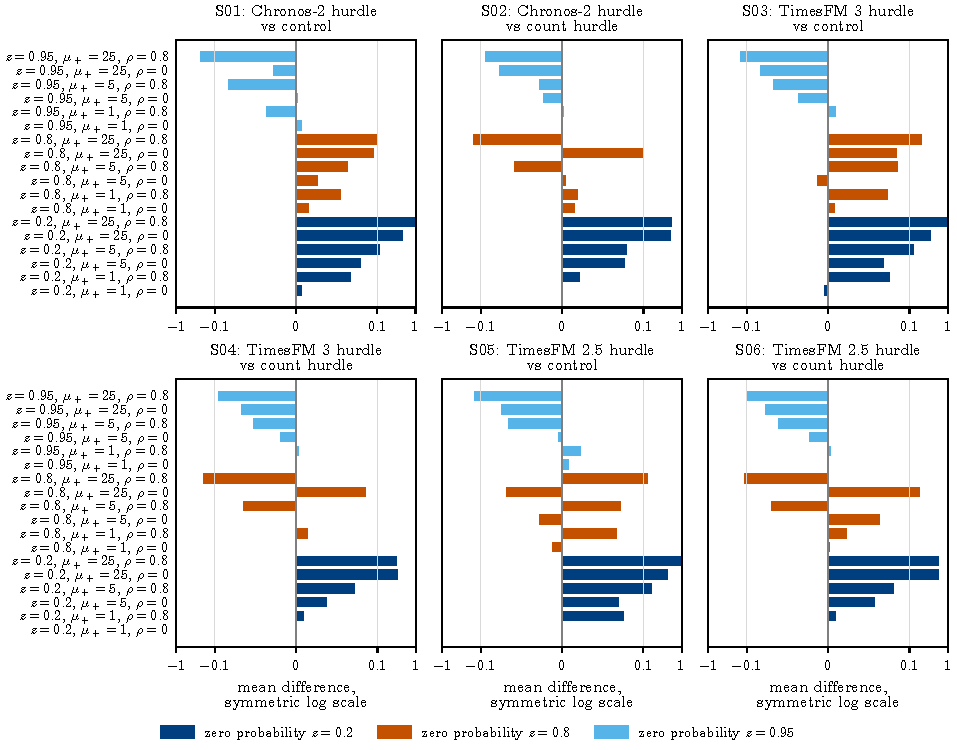
\includegraphics[width=\textwidth]{fig-s2-synthetic-cells}
\caption{The six synthetic comparisons, cell by cell at horizon 30: the mean paired difference over 30
replicates in each of the 18 generator cells, labeled by zero probability $z$, positive mean $\mu_{+}$ and
persistence $\rho$. Negative favors the hurdle variant. The family tests pool the cells with equal weight
(Table~\ref{tab:s2syn}); the cells carry no test.}
\label{fig:s2cells}
\end{figure}

\paragraph{The dynamic-occurrence post-hoc, the detail.} The analysis summarized in
Section~\ref{sec:discussion} is post-hoc. It was computed on 2026-10-16 from the saved forecasts of both
runs, after the registered scores were seen, with no registered status; it adds no test to E01 to E18 or
S01 to S06 and replaces nothing in them, and no model was run. The registered hurdle's occurrence estimate is constant over
the horizon and ignores persistence; the registered \texttt{dynamic\_count} baseline carries a dynamic one,
the discounted Beta-Bernoulli with discount 0.98. The wrapper tested here is the registered hurdle with the
Jeffreys $p$ replaced by $p_{\text{dyn}} = a_B / (a_B + b_B)$, read from \texttt{dynamic\_count}'s saved law
for the same day, with $G_+$ the model's saved completed positive law exactly as the registered hurdle uses
it; where \texttt{dynamic\_count} falls back to \hc{} by its registered rule, in 10 of the 627 npm windows
at each horizon and 501 of the 1,620 grid windows, the wrapper is the registered hurdle. Each wrapper is
compared with the model's completed control, the model's registered hurdle, \texttt{dynamic\_count} (whose
occurrence it shares on every day, so the positive law alone differs) and \hc{}: 24 tests on npm, DE01 to
DE24, and 12 on the grid, DS01 to DS12, each family with the registered settings and its own
Benjamini-Hochberg adjustment at $q = 0.05$. Before any output was written the command verified every
checkpoint hash, rebuilt both registered families byte for byte from the saved scores, and reproduced the
registered hurdle exactly in every window when given the Jeffreys $p$. Table~\ref{tab:s2dyn} gives the rows
against the completed control and the registered hurdle, and Table~\ref{tab:s2dynrest} the rows against
\texttt{dynamic\_count}, whose occurrence each wrapper shares on every day, and against \hc{};
Table~\ref{tab:s2dynparts} gives the three accounting parts of the wrappers and their references on the
grid at horizon 30, each an equal-block mean over the full horizon, and the parts sum to \qs{}.

\begin{table}[htbp]
\centering\footnotesize\setlength{\tabcolsep}{3.5pt}
\caption{Post-hoc. The model's completed positive law wrapped with \texttt{dynamic\_count}'s occurrence,
against the model's completed control and against the model's registered fixed-occurrence hurdle, on npm
(DE rows, 209 series) and the grid (DS rows, 30 replicate blocks at horizon 30). Differences are wrapper
minus reference \qs{}; negative favors the wrapper. The interval is the pointwise 95 percent percentile
interval from 20,000 entity bootstrap replicates; $p$ is Benjamini-Hochberg adjusted once over the 24 npm or
the 12 grid post-hoc tests. ``L / T / H'' counts the series or blocks where the wrapper is lower, tied or
higher. The npm means are unscaled and carried by \texttt{aggregate-error}; a median of order $10^{-17}$ is
floating-point residue.}
\label{tab:s2dyn}
\begin{tabular}{lllrrcrcl}
\toprule
ID & Model & Reference & $h$ & Mean & 95\% interval & Median & L / T / H & Adjusted $p$ \\
\midrule
DE01 & Chronos-2 & completed & 7 & 77.33 & [-0.008112, 231.6] & -0.009524 & 116 / 5 / 88 & 0.24 \\
DE04 & Chronos-2 & fixed hurdle & 7 & -74.67 & [-223.6, -0.148] & -0.001058 & 106 / 6 / 97 & 0.203 \\
DE05 & Chronos-2 & completed & 30 & 26.03 & [-0.05339, 77.77] & -0.005679 & 126 / 4 / 79 & 0.112 \\
DE08 & Chronos-2 & fixed hurdle & 30 & -64.21 & [-191.9, -0.2468] & -0.007901 & 138 / 3 / 68 & $1.64 \times 10^{-6}$ \\
DE09 & TimesFM 3 & completed & 7 & 93.25 & [-0.0469, 279.4] & 0.004233 & 80 / 15 / 114 & 0.121 \\
DE12 & TimesFM 3 & fixed hurdle & 7 & -83.65 & [-250.3, -0.2098] & 0 & 102 / 5 / 102 & 0.367 \\
DE13 & TimesFM 3 & completed & 30 & 54.04 & [-0.09206, 161.8] & -0.0002469 & 106 / 11 / 92 & 0.838 \\
DE16 & TimesFM 3 & fixed hurdle & 30 & -74.49 & [-222.2, -0.4329] & -0.004938 & 131 / 7 / 71 & $6.88 \times 10^{-6}$ \\
DE17 & TimesFM 2.5 & completed & 7 & 82.61 & [0.1723, 247] & 0.002116 & 95 / 6 / 108 & 0.0787 \\
DE20 & TimesFM 2.5 & fixed hurdle & 7 & -171.3 & [-513, -0.2688] & 0.002116 & 93 / 8 / 108 & 0.794 \\
DE21 & TimesFM 2.5 & completed & 30 & 28.84 & [0.08909, 85.83] & $-5.551 \times 10^{-17}$ & 105 / 3 / 101 & 0.471 \\
DE24 & TimesFM 2.5 & fixed hurdle & 30 & -81.49 & [-242.9, -0.5095] & -0.004198 & 124 / 5 / 80 & 0.000642 \\
\midrule
DS01 & Chronos-2 & completed & 30 & 0.0278 & [-0.008979, 0.06239] & 0.04308 & 10 / 0 / 20 & 0.0959 \\
DS04 & Chronos-2 & fixed hurdle & 30 & -0.05819 & [-0.09786, -0.02406] & -0.04727 & 21 / 0 / 9 & 0.00823 \\
DS05 & TimesFM 3 & completed & 30 & 0.02813 & [-0.01113, 0.0638] & 0.02883 & 10 / 0 / 20 & 0.0959 \\
DS08 & TimesFM 3 & fixed hurdle & 30 & -0.05849 & [-0.09728, -0.02412] & -0.04468 & 21 / 0 / 9 & 0.00823 \\
DS09 & TimesFM 2.5 & completed & 30 & 0.03462 & [-0.004804, 0.07104] & 0.04275 & 7 / 0 / 23 & 0.0439 \\
DS12 & TimesFM 2.5 & fixed hurdle & 30 & -0.05307 & [-0.0902, -0.02105] & -0.03688 & 20 / 0 / 10 & 0.00823 \\
\bottomrule
\end{tabular}
\end{table}

The dynamic occurrence shrinks the loss and removes four of the five rejections against the substitution,
and it still never beats the model's own zero mass at $q = 0.05$. Against the completed control no npm row
rejects, with adjusted $p$ from 0.0787 to 0.838, where the registered hurdle had two rejections against it;
every mean difference is still positive, 26.03 to 93.25 against 90.24 to 253.9 for the registered hurdle,
and by rank sum the typical series leans to the Chronos-2 wrapper at both horizons, lower on 116 and 126 of
209 series, and to the control for both TimesFM models. On the grid two of the three rows against the
control no longer reject (DS01 and DS05, adjusted $p$ 0.0959) and the third, TimesFM 2.5 (DS09, adjusted $p$
0.0439), still rejects against the wrapper; the means are 0.0278 to 0.03462 against 0.08599 to 0.08769
registered, and every interval now includes zero. Against the registered fixed-occurrence hurdle the wrapper
is better at horizon 30 everywhere: on npm all three models reject in its favor, lower on 124 to 138 of 209
series, and on the grid all three reject in its favor, lower in 20 or 21 of 30 blocks (adjusted $p$
0.00823); at horizon 7 on npm no row rejects. Against \texttt{dynamic\_count} itself all six npm rows reject
in the wrapper's favor and all three grid rows reject against it, \texttt{dynamic\_count} being lower in 26
to 28 of 30 blocks; against \hc{} all six npm rows reject in the wrapper's favor and on the grid none of the
three rejects, where the registered S02 and S06 rejected against the hurdle. The accounting (Appendix
Table~\ref{tab:s2dynparts}) says where the remaining loss sits: on the grid the wrapper has the lowest
zero-day part of every forecaster, 0.3653 to 0.3879, while its positive-day underprediction part stays at
1.303 to 1.37 against 1.029 to 1.085 for the completed controls and 1.088 for \texttt{dynamic\_count}, whose
occurrence is the same on every day. With the occurrence held equal, the foundation models' positive laws
underpredict the grid's positive days more than the dynamic count's negative binomial does: on the grid the
remaining loss is the positive law.

\begin{table}[htbp]
\centering\footnotesize\setlength{\tabcolsep}{3.5pt}
\caption{Post-hoc. The wrapper against \texttt{dynamic\_count} and against \hc{}, on npm (209 series) and
the grid (30 blocks at horizon 30), with the columns and adjustment of Table~\ref{tab:s2dyn}. The npm means
are unscaled and carried by \texttt{aggregate-error}.}
\label{tab:s2dynrest}
\begin{tabular}{lllrrcrcl}
\toprule
ID & Model & Reference & $h$ & Mean & 95\% interval & Median & L / T / H & Adjusted $p$ \\
\midrule
DE02 & Chronos-2 & count hurdle & 7 & -5,165 & [-15,402, -32.05] & -0.009524 & 122 / 3 / 84 & $2.69 \times 10^{-8}$ \\
DE03 & Chronos-2 & dynamic count & 7 & -6,371 & [-19,017, -32.41] & -0.01376 & 123 / 26 / 60 & $3.1 \times 10^{-11}$ \\
DE06 & Chronos-2 & count hurdle & 30 & -6,627 & [-19,794, -31.46] & -0.08272 & 176 / 2 / 31 & $6.44 \times 10^{-26}$ \\
DE07 & Chronos-2 & dynamic count & 30 & -7,219 & [-21,554, -32.27] & -0.02988 & 143 / 18 / 48 & $1.07 \times 10^{-19}$ \\
DE10 & TimesFM 3 & count hurdle & 7 & -5,499 & [-16,403, -32.2] & -0.008466 & 120 / 1 / 88 & $1.66 \times 10^{-6}$ \\
DE11 & TimesFM 3 & dynamic count & 7 & -6,705 & [-20,020, -32.3] & -0.002116 & 107 / 41 / 61 & $6.81 \times 10^{-9}$ \\
DE14 & TimesFM 3 & count hurdle & 30 & -6,866 & [-20,501, -31.93] & -0.09012 & 171 / 5 / 33 & $6.44 \times 10^{-26}$ \\
DE15 & TimesFM 3 & dynamic count & 30 & -7,458 & [-22,272, -32.36] & -0.03556 & 142 / 36 / 31 & $8.61 \times 10^{-22}$ \\
DE18 & TimesFM 2.5 & count hurdle & 7 & -6,018 & [-17,965, -32.15] & -0.008466 & 117 / 1 / 91 & $2.94 \times 10^{-5}$ \\
DE19 & TimesFM 2.5 & dynamic count & 7 & -7,224 & [-21,578, -32.25] & 0 & 95 / 32 / 82 & $2.94 \times 10^{-5}$ \\
DE22 & TimesFM 2.5 & count hurdle & 30 & -6,999 & [-20,911, -30.68] & -0.07654 & 168 / 4 / 37 & $5.15 \times 10^{-24}$ \\
DE23 & TimesFM 2.5 & dynamic count & 30 & -7,592 & [-22,681, -31.8] & -0.0284 & 135 / 29 / 45 & $6.4 \times 10^{-18}$ \\
\midrule
DS02 & Chronos-2 & count hurdle & 30 & -0.006081 & [-0.06427, 0.05495] & $5.487 \times 10^{-5}$ & 15 / 0 / 15 & 0.734 \\
DS03 & Chronos-2 & dynamic count & 30 & 0.09152 & [0.05951, 0.131] & 0.08335 & 3 / 0 / 27 & $9.84 \times 10^{-5}$ \\
DS06 & TimesFM 3 & count hurdle & 30 & -0.03699 & [-0.08884, 0.01326] & -0.03181 & 20 / 0 / 10 & 0.128 \\
DS07 & TimesFM 3 & dynamic count & 30 & 0.0606 & [0.03767, 0.08388] & 0.05156 & 4 / 0 / 26 & 0.000301 \\
DS10 & TimesFM 2.5 & count hurdle & 30 & 0.008012 & [-0.04943, 0.06357] & 0.02626 & 14 / 0 / 16 & 0.734 \\
DS11 & TimesFM 2.5 & dynamic count & 30 & 0.1056 & [0.07495, 0.1372] & 0.09752 & 2 / 0 / 28 & $9.84 \times 10^{-5}$ \\
\bottomrule
\end{tabular}
\end{table}

\begin{table}[htbp]
\centering\small
\caption{Post-hoc. The three exact accounting parts on the synthetic grid at horizon 30, equal-block means
over the full horizon, for each model's dynamic-occurrence wrapper, its registered hurdle and its completed
control, and for \texttt{dynamic\_count}, \hc{} and the oracle. The parts sum to \qs{}.}
\label{tab:s2dynparts}
\begin{tabular}{lrrrr}
\toprule
Variant & \qs{} & Zero days & Positive, overprediction & Positive, underprediction \\
\midrule
chronos2\_dyn & 1.813 & 0.3682 & 0.0847 & 1.36 \\
chronos2\_hurdle & 1.871 & 0.4046 & 0.08819 & 1.378 \\
chronos2\_completed & 1.785 & 0.5798 & 0.1201 & 1.085 \\
timesfm3\_dyn & 1.782 & 0.3879 & 0.09111 & 1.303 \\
timesfm3\_hurdle & 1.84 & 0.4294 & 0.09493 & 1.316 \\
timesfm3\_completed & 1.754 & 0.6014 & 0.1231 & 1.029 \\
timesfm2p5\_dyn & 1.827 & 0.3653 & 0.09171 & 1.37 \\
timesfm2p5\_hurdle & 1.88 & 0.3947 & 0.09467 & 1.39 \\
timesfm2p5\_completed & 1.792 & 0.624 & 0.1334 & 1.035 \\
dynamic\_count & 1.721 & 0.5214 & 0.1114 & 1.088 \\
hurdle\_count\_28 & 1.819 & 0.5923 & 0.118 & 1.108 \\
oracle & 1.648 & 0.4817 & 0.1102 & 1.056 \\
\bottomrule
\end{tabular}
\end{table}
